\documentclass[11pt]{article}
\usepackage[a4paper,margin=24mm]{geometry}
\usepackage[T1]{fontenc}
\usepackage{lmodern,microtype,amsmath,amssymb,amsthm,mathtools}
\usepackage{booktabs,array,graphicx,xcolor,enumitem,fancyhdr}
\usepackage[colorlinks=true,linkcolor=teal!65!black,citecolor=teal!65!black,urlcolor=teal!65!black]{hyperref}
\definecolor{ink}{HTML}{153044}\definecolor{accent}{HTML}{087F8C}
\setlength{\parindent}{0pt}\setlength{\parskip}{5pt}\setlength{\headheight}{15pt}
\pagestyle{fancy}\fancyhf{}
\fancyhead[L]{\small Quantum mechanics and general relativity: matter limits}
\fancyhead[R]{\small Logan Voss}\fancyfoot[C]{\thepage}
\newtheorem{theorem}{Theorem}[section]
\newtheorem{proposition}[theorem]{Proposition}
\newtheorem{lemma}[theorem]{Lemma}
\newtheorem{corollary}[theorem]{Corollary}
\newcommand{\Tr}{\operatorname{Tr}}\newcommand{\dd}{\mathrm d}
\newcommand{\R}{\mathbb R}\newcommand{\Lip}{\operatorname{Lip}}
\newcommand{\vol}{\operatorname{vol}}\newcommand{\Div}{\operatorname{div}}
\hypersetup{pdftitle={On Quantum Mechanics and General Relativity: Controlled Matter-Continuum Limits},pdfauthor={Logan Voss},pdfsubject={A quantitative large-population matter continuum at fixed geometric Galerkin cutoff}}
\begin{document}
\hypersetup{pageanchor=false}
\begin{titlepage}
\vspace*{10mm}
{\color{accent}\small\scshape Research edition 3.0}\par\vspace{9mm}
{\color{ink}\Huge\bfseries On Quantum Mechanics\par and General Relativity}\par\vspace{8mm}
{\Large Logan Voss}\par\vspace{8mm}
{\large Controlled Matter-Continuum Limits}\par\vspace{10mm}
\hrule\vspace{6mm}
\textbf{The result.} An explicitly augmented quantum regulator converges, on a regular finite time interval, to covariant state-fluid matter with reciprocal response through a fixed finite geometric basis.
\[
\boxed{\mathfrak D_n(t)\le e^{Ct}
\left[\mathfrak D_n(0)+\frac{B^2t}{n^2}\right].}
\]
The collective internal state converges in trace norm, the relativistic parcel acquires the proper-flow quantum clock, and strong current estimates control the required quadratic contact functional.
\[
\boxed{\delta_J=O(\ell^{4/5}),\qquad
\text{contact error}=O(\ell^{4/5})}
\]
for one explicit sufficient diagonal with all fixed-cutoff constants retained.
\par\vspace{4mm}
\textbf{The boundary.} The nonlinear geometric Galerkin cutoff is held fixed. A separate linearized theorem removes the spatial lattice on an exact Einstein-dust background. Neither result establishes unrestricted nonlinear Einstein-constraint convergence or a fixed-coupling quantum-gravity ultraviolet limit.
\vfill
{\small November 13, 2026\par
AI-assisted research, including derivation, verification, formalization, and editing. Calculations and independent review preceded public authoring. The evidence is mathematical and synthetic; no experimental measurements are reported.}\par
\end{titlepage}
\hypersetup{pageanchor=true}

\begin{abstract}
We derive a controlled connection from an augmented quantum regulator to the covariant state-fluid matter model of the preceding research, while retaining a fixed finite geometric field basis. A bounded-observable algebra yields an explicit finite-time concentration estimate for polynomial Hamiltonians and positive square-root terms. A resolvent argument controls both Heisenberg generators and the Fréchet derivatives that define actual sources and stress. Symmetric-probe identities give trace-norm propagation of chaos. The collective relativistic mass produces the proper-time Schrödinger multiplier and the required worldline action. Reciprocal material quadrature then converges before caustics, and strong operator-valued current estimates preserve a specified ordered contact functional. We state the population, phase-space, Fourier, internal, and mollifier dependencies and give a sufficient diagonal. Internal oscillator removal is a separate ordered estimate with uniform moment and common-interval hypotheses. A corrected whole-field linearized theorem also removes a physical spatial lattice on an exact Einstein-dust background. Fixed-occupancy energy, mixed-state, multistream, nonlinear-mass, and weak-current controls show why the assumptions cannot be omitted. The resulting endpoint is a controlled matter continuum with projected geometric equations; the unrestricted nonlinear geometric cutoff and full Einstein constraints remain open.
\end{abstract}
\setcounter{tocdepth}{1}\tableofcontents
\newpage

\section{The exact endpoint and the required augmentation}
The previous quantum cell~\cite{Voss2} quantizes a shape matrix and an independent oscillator:
\[
\mathcal H=L^2(\mathbb H^2,\dd\vol_G)\otimes L^2(\R),
\qquad
H=-\frac{\hbar^2}{2I}\Delta_G+H_M^{\mathrm{ex}}.
\]
Its target metric and selected interaction are
\begin{equation}\label{eq:target}
G=\frac{\dd u^2+\dd v^2}{v^2},\qquad
M=\frac1v\begin{pmatrix}1&u\\u&u^2+v^2\end{pmatrix},
\qquad
H_M^{\mathrm{ex}}=\frac{\hbar\omega}{2}\widehat R^TM^{-1}\widehat R
-\frac{\hbar\omega}{2}I.
\end{equation}
The canonical quadratures satisfy $[\widehat Q,\widehat P]=i$ in calibrated units. Refining a grid of $(u,v)$ values improves the representation of one quantum shape. It does not create physical positions, transport momentum, material labels, or a spacetime number current.

The present microscopic family adds physical parcels, symmetric internal populations, spatial shape couplings, and a common extensive scaling. It retains the selected local interaction, but does not pretend that the additional transport architecture follows from a one-cell Hamiltonian.

\begin{center}\small
\begin{tabular}{@{}>{\raggedright\arraybackslash}p{0.16\textwidth}>{\raggedright\arraybackslash}p{0.37\textwidth}>{\raggedright\arraybackslash}p{0.39\textwidth}@{}}
\toprule
Parameter & Meaning & Treatment\\\midrule
$N$ & Collective population and geometric-action scale & Large-population concentration\\
$\ell$ & Physical material-label mesh & Nonlinear matter continuum\\
$\eta$ & Current smoothing width & Strong current/contact limit\\
$d$ & Internal oscillator cutoff & Separate ordered removal\\
Fourier/phase cutoffs & Positive canonical approximants and localization & Explicit coefficient error, then population selection\\
$L$ & Number of geometric field modes & Fixed in the nonlinear theorem\\
$a$ & Spatial mesh in the separate tangent theorem & Removed with an explicit smooth-field bound\\\bottomrule
\end{tabular}
\end{center}

\subsection{Regularity and physical scaling}
Fix $L,d$, a positive rest energy $m_0$, and a prescribed smooth Lorentzian $2+1$ background. Here $d$ denotes the internal cutoff; the spatial and material dimension is denoted separately by $d_x=2$. The retained shape coefficients are dynamical. Work on a common finite interval $[0,T]$ on which the classical phase trajectories stay in a compact physical patch, target heights are positive, proper-clock factors have a positive margin, and the material map is a smooth diffeomorphism with positive Jacobian margin. The occupied material density is smooth and bounded away from zero.

For material weights $\mu_j\simeq n_0(a_j)\ell^2$, use
\[
K_j=\operatorname{round}(N\mu_j),\qquad
K_{\min}\ge c_0N\ell^2
\]
when $N$ is sufficiently large. Scale the geometric action by $N$ and normalize action and energy per $N$. A physical cell of volume $v_{\mathrm c}$ then has geometric inertia proportional to $Nfv_{\mathrm c}$ and population proportional to $Nn_0v_{\mathrm c}$.

This is a collective weak-coupling family. It is not an ultraviolet limit at fixed $\hbar$, fixed Newton coupling, and fixed occupancy. Rounding changes both weights and subsequent trajectories; both effects enter the estimates.

For each integer population, the quantum estimate compares with its matching classical Hamiltonian using the same rounded weights $K_j/N$. Coefficient bounds are taken uniformly over the bounded rounding-ratio range. A separate classical rounding-stability estimate then reaches the common fluid weights $\mu_j$. Constants are chosen after the finite coefficient approximation is fixed and before selecting population; they do not conceal a population-dependent $A_\ell$.

\begin{theorem}[Controlled matter endpoint]\label{thm:main}
In the stated regular fixed-$L,d$ regime, there are self-adjoint finite quantum regulators and well-prepared states whose bounded phase-space observables, fixed-probe marginals, matter sources, and mollified currents converge to the state-fluid matter quantities coupled reciprocally to the retained geometric modes. A positive zero-shift realization exists. The current-squared functional converges in a specified order under strong current control.

The limiting matter equations are generated by the covariant state-fluid action, while the geometric equations remain projected onto the fixed basis. This is a dynamical and source-convergence statement, not a quantum-action $\Gamma$-convergence theorem. It does not imply unrestricted pointwise twist closure or the full Einstein equations.
\end{theorem}

The proof is composed below from a quantum concentration theorem, reciprocal material quadrature, and strong current control. At fixed cutoffs the regular interval is nonempty for regular initial data: in material coordinates the system is a smooth ODE on mode variables and regular label maps, with no label derivatives in its right-hand side. The estimates are local in this regular regime, before caustics or chart departure.

\section{A bounded-algebra quantum concentration theorem}
Let $Y_1^{(n)},\ldots,Y_m^{(n)}$ be self-adjoint operators with $\|Y_j\|\le1$. Let their real classical coordinates satisfy $|y_j|\le1$ on a compact embedded Poisson phase space. Use the Heisenberg convention
\[
\Pi_{ij}(y)=\{y_j,y_i\}.
\]
Assume the finite regulator algebra obeys
\begin{equation}\label{eq:basic}
\frac{in}{\hbar}[Y_i,Y_j]=\Pi_{ij}(Y)+R_{ij,n},
\quad \|R_{ij,n}\|\le\frac{r_0}{n},
\quad \|[Y_i,Y_j]\|\le\frac{\kappa_0}{n},
\end{equation}
with fixed ordered polynomials $\Pi_{ij}$. The substitution may have an ordering discrepancy; the scaled commutator $(in/\hbar)[Y_i,Y_j]$ is Hermitian and the remainder accounts for that discrepancy. The raw commutator is anti-Hermitian.

For an ordered polynomial $P=\sum_\alpha c_\alpha y_{\alpha_1}\cdots y_{\alpha_{k_\alpha}}$, set
\[
M_P=\sum_\alpha|c_\alpha|,
\qquad L_P=\sum_\alpha|c_\alpha|k_\alpha.
\]
For normalized $\Psi$ and
\begin{equation}\label{eq:D}
\mathfrak D_n=\sum_j\|(Y_j-y_j)\Psi\|^2,
\end{equation}
finite telescoping gives
\begin{equation}\label{eq:tel}
\|(P(Y)-P(y))\Psi\|\le L_P\sqrt{\mathfrak D_n}.
\end{equation}
To prove this, replace a monomial's factors from right to left. Every term has a bounded operator prefix, one deviation factor acting directly on $\Psi$, and a scalar suffix. No independence assumption or unproved commutation is used.

Leibniz expansion of \eqref{eq:basic} gives
\begin{equation}
\frac{in}{\hbar}[P(Y),Y_j]=G_{Pj}(Y)+R_{Pj,n},
\qquad \|R_{Pj,n}\|\le r_0L_P/n,
\end{equation}
where the explicitly constructed scalar symbol is $G_{Pj}(y)=\{y_j,P\}$. A second expansion gives
\begin{equation}\label{eq:polycomm}
\|[P(Y),Q(Y)]\|\le\kappa_0L_PL_Q/n.
\end{equation}
These coefficient bounds may be large; they are retained rather than silently assumed uniform in a growing cutoff.

\subsection{The positive square-root lemma}
\begin{lemma}\label{lem:sqrt}
Let $B=B(Y)$ be self-adjoint with $B\ge m_0^2I$, and let $b=B(y)\ge m_0^2$, $m_0>0$. Define $C_n=(in/\hbar)[B,Y_j]$ and $c=G_{Bj}(y)$. Then
\begin{equation}\label{eq:sqrtbound}
\begin{split}
\left\|\left(\frac{in}{\hbar}[\sqrt B,Y_j]-\frac{c}{2\sqrt b}\right)\Psi\right\|
\le{}&\frac{\|(C_n-c)\Psi\|}{2m_0}
+\frac{|c|\|(B-b)\Psi\|}{4m_0^3}\\
&+\frac{\|[C_n,B]\|}{8m_0^3}.
\end{split}
\end{equation}
\end{lemma}
\begin{proof}
Positive functional calculus gives
\[
[\sqrt B,Y_j]=\frac1\pi\int_0^\infty
t^{1/2}(B+t)^{-1}[B,Y_j](B+t)^{-1}\dd t.
\]
With $R=(B+t)^{-1}$ and $r=(b+t)^{-1}$,
\[
RC_nR-cr^2=R^2(C_n-c)+R[C_n,R]+c(R^2-r^2).
\]
Use $[C_n,R]=-R[C_n,B]R$ and $R-r=-rR(B-b)$. Their three norm factors are $(m_0^2+t)^{-2}$, $(m_0^2+t)^{-3}$, and $2(m_0^2+t)^{-3}$. The exact integrals are
\[
\frac1\pi\int_0^\infty\frac{t^{1/2}}{(m_0^2+t)^2}\dd t=\frac1{2m_0},
\qquad
\frac1\pi\int_0^\infty\frac{t^{1/2}}{(m_0^2+t)^3}\dd t=\frac1{8m_0^3}.
\]
This proves \eqref{eq:sqrtbound}. Finite regulators have no remaining operator-domain issue in this step.
\end{proof}

Writing $G=G_{Bj}$, one explicit generator bound is $a_j\sqrt{\mathfrak D_n}+b_j/n$, with
\begin{align}
a_j&=\frac{L_G}{2m_0}+\frac{M_GL_B}{4m_0^3},\\
b_j&=\frac{r_0L_B}{2m_0}
+\frac{\kappa_0L_GL_B+2M_Br_0L_B}{8m_0^3}.
\end{align}
The last numerator follows by splitting $C_n=G(Y)+R_{Bj,n}$ and applying \eqref{eq:polycomm}.

\subsection{Actual Hamiltonian source variations}
The same integral represents the Fréchet derivative $D\sqrt B[C]$ for a self-adjoint variation $C$. The identical estimate applies with $C=\delta B$, $c=\delta b$. If $\delta B$ has the stated polynomial bounds, derivatives of the actual normalized quantum Hamiltonian converge to derivatives of its limiting symbol. This controls scalar sources and metric/stress variations; the classical observables are not assigned afterwards to fit a desired equation.

In a matrix eigenbasis of $B$, the derivative has entries $C_{ij}/(\sqrt{b_i}+\sqrt{b_j})$, which supplies an independent numerical control.

\begin{theorem}[Finite-time concentration]\label{thm:conc}
Let
\[
K_n=P_0(Y)+\sum_\ell w_\ell\sqrt{B_\ell(Y)},
\qquad B_\ell(Y)\ge m_\ell^2I,\quad B_\ell(y)\ge m_\ell^2>0.
\]
Assume $K_n$ is self-adjoint, the weights are real, and its classical symbol $k(y)$ is real. Evolve
$i\hbar\partial_t\Psi_n=nK_n\Psi_n$ and the classical Hamilton equations generated by $k$.
Sum the per-term bounds above, including $|w_\ell|$, and put
$a=(\sum_ja_j^2)^{1/2}$, $b=(\sum_jb_j^2)^{1/2}$, $C=2a+1$. Then
\begin{equation}\label{eq:concentration}
\boxed{\mathfrak D_n(t)\le e^{Ct}
\left[\mathfrak D_n(0)+\frac{b^2t}{n^2}\right].}
\end{equation}
\end{theorem}
\begin{proof}
Exact Schrödinger differentiation of \eqref{eq:D}, followed by Cauchy--Schwarz and the generator estimates, gives
\[
\mathfrak D_n'\le2\sqrt{\mathfrak D_n}
(a\sqrt{\mathfrak D_n}+b/n)
\le C\mathfrak D_n+b^2/n^2.
\]
Integrating the scalar differential inequality proves the displayed bound.
\end{proof}
For fixed regulator data, the constants do not depend on population. Smooth time-dependent coefficients are allowed when their bounds are uniform on $[0,T]$. This theorem requires linear unitary self-adjoint evolution. It does not assert positivity for arbitrary polynomial terms or signed weights; the physical zero-shift kinetic and mass construction supplies a positive realization.

\section{Prepared states and the proper quantum clock}
\subsection{Canonical coordinates and positive approximants}
Clock/shift matrices with
\[
UV=e^{-2\pi i/r}VU
\]
give bounded real and imaginary coordinate components. With $r=cn$ for fixed integer $c>0$, exact Weyl multiplication yields \eqref{eq:basic}, with conservative constants
\[
\kappa_0=\max(2\pi/c,2),\qquad
r_0=\frac{2\pi^2}{c^2\hbar}
\]
and the corresponding canonical-area normalization. The negative phase fixes the positive physical canonical orientation. Physical coordinates agree with these periodic representatives only in the specified interior patch.

A periodized Gaussian
\[
\phi_r(j)=Z_r^{-1/2}\sum_{k\in\mathbb Z}
\exp[-\pi(j+kr)^2/r]
\]
is invariant under the unitary discrete Fourier transform. For four real clock/shift observables centered at $(1,0,1,0)$, its deviation is $4(1-\mathrm{Re}\langle U\rangle)$. The elementary bounds $1-\cos\theta\le\theta^2/2$ and $\langle j^2\rangle\le50r$ imply
\[
\mathfrak D_{0,\mathrm{canonical}}\le400\pi^2/r,\qquad r\ge4.
\]
The moment estimate follows by bounding the periodized amplitude by $\sqrt5$ times its central Gaussian, using $Z_r\ge(\sqrt r/2)e^{-\pi/2}$, and bounding the Gaussian second-moment sum by $r^{3/2}$. Nearest-grid translations add $O(r^{-2})$ center error.

Only finite positive Fourier/polynomial approximants are used. A smooth periodic positive extension $h_d^R$ equals the projected selected oscillator near the physical patch. If a Hermitian Fourier polynomial $p_{d,F}$ has $C^r$ error at most $\delta_{\mathrm{reg}}$, then $p_{d,F}+\delta_{\mathrm{reg}}I\ge0$, with value error at most $2\delta_{\mathrm{reg}}$ and derivative error at most $\delta_{\mathrm{reg}}$. Metric and momentum representatives are treated similarly. The kinetic ordering $\sum P_ag^{ab}_{\mathrm{poly}}P_b$ preserves positivity.

At fixed remaining cutoffs, classical vector-field and trajectory errors are bounded by $C_{\mathrm{reg}}\delta_{\mathrm{reg}}$ and $C_T\delta_{\mathrm{reg}}$. They are included in the final diagonal. Large coefficient sums, including possible growth from Hermitian Fourier expansion, stay inside the actual constants of Theorem~\ref{thm:conc}. No smooth-series or degree-uniform extension is assumed.

\subsection{Propagation of pure internal-state closure}
For an HS-orthonormal Hermitian basis $B_\alpha$ of the $d$-level internal system, including $I/\sqrt d$, define
\[
A_n(B_\alpha)=n^{-1}\sum_{j=1}^n B_\alpha^{(j)}.
\]
The internal Lie commutators have exact size $1/n$. The identity
$\sum_\alpha B_\alpha\otimes B_\alpha=\mathrm{Swap}$ gives, on the symmetric sector,
\[
\sum_\alpha A_n(B_\alpha)^2=1+(d-1)/n.
\]
For a pure target $\rho=|\psi\rangle\langle\psi|$, let
\[
S_n=\sum_\alpha\left\langle
(A_n(B_\alpha)-\Tr\rho B_\alpha)^2\right\rangle,
\qquad \beta_n=1-\Tr(\rho\rho_n^{(1)}).
\]
Then exactly
\begin{equation}\label{eq:chaos}
\boxed{S_n=2\beta_n+\frac{d-1}{n},\qquad
\|\rho_n^{(k)}-\rho^{\otimes k}\|_1\le2\sqrt{k\beta_n}\le\sqrt{2kS_n}.}
\end{equation}
The marginal estimate follows from the union bound for commuting one-particle projectors and the pure-state trace-distance inequality. It applies to fixed $k\le n$, not to convergence of the entire many-body state to a product in norm.

For pure product internal data, $S_n(0)=(d-1)/n$. Together with the canonical preparation this gives an explicit nonempty class with $\mathfrak D_n(0)\le C_{\mathrm{prep}}/n$. The internal degree remains a quantum state governed by its projective-Hilbert Poisson structure.

\subsection{The collective relativistic parcel}
Use units $c=1$ in the relativistic energy and proper-time formulas below.
Use the augmented parcel Hamiltonian
\begin{equation}\label{eq:parcel}
H_n^{\mathrm{parcel}}
=n\sqrt{P_n^2+\left[m_0+A_n(h(q(X_n)))\right]^2}.
\end{equation}
The root argument is at least $m_0^2I$ for nonnegative internal $h$, even when momentum and mass do not commute. The limiting symbol is
\[
E=\sqrt{p^2+\varepsilon^2},
\qquad \varepsilon=m_0+\Tr(\rho h(q(X))).
\]
Its equations are
\begin{equation}\label{eq:properclock}
\dot X=p/E,\qquad
\dot p=-(\varepsilon/E)\Tr(\rho\,\partial_Xh),\qquad
i\hbar\dot\psi=(\varepsilon/E)h\psi
\end{equation}
up to a phase multiplier. Since $\dd\tau/\dd t=\varepsilon/E=\sqrt{1-|\dot X|^2}$, the internal equation is $i\hbar\,\dd\psi/\dd\tau=h\psi$.

For an ADM metric, denote its lapse by $\mathcal N$, distinct from the geometric cutoff $L$:
$h=-\mathcal N^2\dd t^2+\gamma_{ij}(\dd x^i+\beta^i\dd t)(\dd x^j+\beta^j\dd t)$.
The classical Hamiltonian is
$\mathcal N\sqrt{\gamma^{ij}p_ip_j+\varepsilon^2}-\beta^ip_i$.
A variable lapse is covered by the explicit positive ordering
$\sqrt{\mathcal N_{\mathrm{poly}}B\mathcal N_{\mathrm{poly}}}$:
if $\mathcal N_{\mathrm{poly}}\ge\mathcal N_{\min}>0$, its argument is at least
$m_0^2\mathcal N_{\min}^2I$ and its exact classical symbol is
$\mathcal N_{\mathrm{poly}}(y)\sqrt{b(y)}$.
The approximation to the physical lapse $\mathcal N$ is a separate coefficient-consistency error.
The shift is symmetrically ordered. This is a declared ordering, not a uniqueness theorem for quantized covariant matter, and a generic shift need not preserve total positivity.

The collective architecture is essential. In general
\[
\Tr\rho\sqrt{p^2+(m_0+h)^2}
\ne\sqrt{p^2+(m_0+\Tr\rho h)^2}.
\]
At energies $0,2$ with equal probabilities and $m_0=|p|=1$, the left side is $(\sqrt2+\sqrt{10})/2>\sqrt5$. Center-of-mass classicalization alone does not remove this nonlinear mass difference.

\section{Reciprocal parcels become covariant state-fluid matter}
\subsection{The exact material-coordinate action}
The identity $p\cdot\dot X-E=-\varepsilon\,\dd\tau/\dd t$ sends the parcel canonical action to
\[
\int\left[i\hbar\langle\psi|\dd\psi\rangle
-(m_0+\langle h\rangle)\dd\tau\right].
\]
For material labels $a$ with smooth weight $w(a)$, write
$X^\mu(t,a)=(t,X(t,a))$ and
$b(t,a)=\sqrt{-h_{\mu\nu}\dot X^\mu\dot X^\nu}>0$.
The label action is
\begin{equation}\label{eq:labelaction}
S_{\mathrm{mat}}=\int\dd t\,\dd a\,w(a)
\left[i\hbar\langle\psi|\dot\psi\rangle
-b(m_0+\langle H_q(X)\rangle)\right].
\end{equation}
Use periodic material/spatial patches, or interior-localized observables with a smooth extension, when applying the smoothing estimates below; a sharp vacuum boundary would not automatically have the required current regularity.

Before caustics, let $\mathcal J_X=\det D_aX>0$. Define Eulerian quantities at $x=X(t,a)$ by
\[
j^0=w/\mathcal J_X,\qquad j^i=j^0\dot X^i,\qquad
n=j^0b/\sqrt{-h},\qquad u^\mu=\dot X^\mu/b,\qquad
\Psi(t,X)=\psi(t,a).
\]
Changing variables $\dd^2x=\mathcal J_X\dd a$ gives exactly
\[
S_{\mathrm{mat}}=\int\left[
j^\mu i\hbar\langle\Psi|\partial_\mu\Psi\rangle
-\sqrt{-h}\,n(m_0+\langle H_q\rangle)\right]\dd^3x.
\]
The transported measure gives $\partial_\mu j^\mu=0$. Its velocity-potential and Clebsch representation is the covariant state-fluid action
\begin{equation}\label{eq:Brown}
\boxed{S_m=\int\left[
j^\mu\left(\partial_\mu\vartheta+i\hbar\langle\Psi|\partial_\mu\Psi\rangle
+\beta_A\partial_\mu\alpha^A\right)
-\sqrt{-h}\,n(m_0+\langle H_q\rangle)\right]\dd^3x.}
\end{equation}
The state normalization is imposed in the variation. General local material flows require the Clebsch-capable description; one velocity potential alone is a restricted subclass. This is established fluid-action structure~\cite{Brown}, now reached from the stated collective parcel.

\subsection{Reciprocal quadrature, not prescribed shape motion}
Retain a fixed finite smooth basis for the shape field $q_z(x)$, including a constant twist-shift mode. Restrict the selected shape action to it. The kinetic matrix is positive and invertible in the regular region. The common Hamiltonian gives
\begin{equation}\label{eq:feedback}
\dot z=F(z,t)+\int_Aw(a)G(z,\xi(t,a),t)\dd a,\qquad
\dot\xi(t,a)=V(z,\xi(t,a),t),
\end{equation}
where $z$ contains shape coefficients and momenta, and $\xi$ contains parcel position, momentum, and internal variables. Both forces come from the same Hamiltonian.

On midpoint cells of width $\ell$, set $\mu_j=\ell^{d_x} w(a_j)$ and replace the integral by $\sum_j\mu_jG$. Suppose the regular-region Lipschitz constants are $L_F,L_G,L_V$, with $\sum_j\mu_j\le W_*$, and define
\[
Q_T=\frac1{24}\sum_{r=1}^{d_x}
\sup_{[0,T]\times A}
\left\|\partial_{a_r}^2\left[w(a)G(z(t),\xi(t,a),t)\right]\right\|,
\qquad C_T=L_F+W_*L_G+L_V.
\]
\begin{proposition}[Reciprocal material limit]\label{prop:quad}
For
$e_\ell(t)=|z_\ell-z|+\max_j|\xi_j-\xi(t,a_j)|$,
\begin{equation}\label{eq:quad}
\boxed{e_\ell(t)\le e^{C_Tt}e_\ell(0)
+Q_T\ell^2\,\frac{e^{C_Tt}-1}{C_T}.}
\end{equation}
The last factor is $t$ when $C_T=0$.
\end{proposition}
\begin{proof}
Subtract \eqref{eq:feedback} and its quadrature version, adding and subtracting the continuum midpoint samples. The midpoint remainder is at most $Q_T\ell^2$. The other terms are bounded by the three Lipschitz constants, giving an upper Dini derivative
$e_\ell'\le C_Te_\ell+Q_T\ell^2$. Integration gives the result.
\end{proof}
The constant is inspectable: if $A_1,A_2$ bound the first and second label derivatives of $\xi$, a second derivative of $wG$ is bounded by
\[
\|w''\|G_0+2\|w'\|G_1A_1
+\|w\|(G_2A_1^2+G_1A_2).
\]
Differentiating the parcel ODE controls $A_1,A_2$ and the $C^1$ flow error on the common interval. A strict Jacobian margin persists for small mesh. These are nonlinear feedback estimates, rather than sampling an already prescribed shape trajectory.

The matter action and its transport equations have a continuum limit. The geometric equations remain Galerkin equations. Retained-mode or global shift conservation is weaker than the full pointwise twist identity $d(*C)=0$; no local connection reconstruction is inferred from that weaker statement.

\section{Strong quantum currents and the contact interaction}
Weak current convergence cannot pass the required $J_aJ^a$ term. Use an even normalized smooth kernel
$K_\eta(x)=\eta^{-d_x}K(x/\eta)$ with finite second moment and square-integrable derivatives through order two.
Assume the limiting current has the corresponding smoothness, so the symmetric-kernel bias is $O(\eta^2)$.

The classical current reconstruction has the bound
\begin{equation}\label{eq:classcurrent}
\|J_{\ell,\eta}-J\|_2
\le C_T\left[
\eta^2+\ell^2\eta^{-d_x/2-2}
+\delta_{\mathrm{path}}\eta^{-d_x/2-1}
+\delta_{\mathrm{amp}}\eta^{-d_x/2}\right].
\end{equation}
The terms arise from kernel bias, Banach-valued midpoint quadrature, translation, and all amplitude errors. The scaling
$\|\nabla^rK_\eta\|_2=\eta^{-d_x/2-r}\|\nabla^rK\|_2$
fixes the powers. Velocity, proper-clock, volume, and internal-state errors must be included in the amplitude, not discarded.

\subsection{Operator-valued current control}
The internal charge is the collective per-probe quantity, not one probe with unsuppressed intrinsic variance. For commuting position components $\widehat X_j$ and bounded self-adjoint amplitudes $\widehat B_j$, choose
\[
\widehat J_\eta(x)=\sum_j\frac{\mu_j}{2}
\{K_\eta(x-\widehat X_j),\widehat B_j\}.
\]
For a vector $\phi$, the spectral theorem gives
\[
\int\|K_\eta(x-\widehat X_j)\phi\|^2\dd x
=\|K_\eta\|_2^2\|\phi\|^2,
\]
and
\[
\int\|[K_\eta(x-\widehat X_j)-K_\eta(x-X_j)]\Psi\|^2\dd x
\le\|\nabla K_\eta\|_2^2\langle|\widehat X_j-X_j|^2\rangle.
\]
Let the RMS position and amplitude deviations be $\delta_{X,j},\delta_{B,j}$. Expand the first order as $K(B-b)+b(K-K_{\rm cl})$ and the second as $B(K-K_{\rm cl})+K_{\rm cl}(B-b)$. Then
\begin{equation}\label{eq:quantcurrent}
\begin{split}
\|(\widehat J_\eta-J_{{\rm cl},\eta})\Psi\|_{L^2_x\mathcal H}
\le\sum_j\mu_j\bigg[
&\|K_\eta\|_2\delta_{B,j}\\
&+\frac{\|\widehat B_j\|+|b_j|}{2}
\|\nabla K_\eta\|_2\delta_{X,j}\bigg].
\end{split}
\end{equation}
No independence between parcels or commutation of $\widehat B_j$ and $\widehat X_j$ is assumed. A symmetrized velocity/charge amplitude is handled by the same product telescoping, with its actual norms retained.

For the weighted contact functional specify
\[
\widehat A_a=\widehat\lambda\widehat J_a,\qquad
\widehat{\mathcal Q}=h^{ab}\widehat A_a^\dagger\widehat A_b.
\]
If $\widehat\lambda$ is bounded and its RMS error is controlled, write
$\|(\widehat A-A)\Psi\|_{L^2_x\mathcal H}=\delta_A$,
$A_a=\lambda J_a$. Cauchy--Schwarz yields
\begin{equation}\label{eq:contact}
\boxed{\int\left|\langle\widehat{\mathcal Q}\rangle
-\lambda^2h^{ab}J_aJ_b\right|\dd x
\le\|h^{-1}\|_\infty\delta_A(2\|\lambda J\|_2+\delta_A).}
\end{equation}
This controls a declared ordering. Another noncommuting order is not silently identified with it, and scalar--connection dualization is not asserted to be an exact identity of the finite-population quantum theory.

\subsection{One sufficient diagonal}
In two material dimensions, the combined estimate is
\begin{equation}\label{eq:combinedcurrent}
\delta_J\le C_T\left[
\eta^2+\ell^2\eta^{-3}
+\delta_{\mathrm{path}}\eta^{-2}
+\delta_{\mathrm{amp}}\eta^{-1}
+\frac1{N\ell^2\eta}\right].
\end{equation}
Path and amplitude errors include quantum RMS, coefficient approximation, reciprocal quadrature, and the trajectory change caused by count rounding. The last term is the direct rounding-weight error.

Choose $0<s\le1$, $\ell=s^5$, and $\eta=s^2$. First fix the positive coefficient approximation so that its induced physical path and amplitude errors are at most $s^8$, including the required kernel factors. This fixes the actual finite polynomial coefficients. At fixed geometric and internal cutoffs, absorb all resulting preparation, evolution, and physical-observable factors into $A_\ell\ge1$, independent of the population subsequently chosen:
\[
\delta_{\mathrm q}\le\frac{A_\ell}{\sqrt{N\ell^2}}.
\]
Set
\begin{equation}\label{eq:diag}
\ell=s^5,\qquad\eta=s^2,\qquad
N\ge A_\ell^2s^{-26},\qquad0<s\le1.
\end{equation}
Then $\delta_{\mathrm q}\le s^8$. The leading terms satisfy
\[
\eta^2=s^4,\qquad
\ell^2\eta^{-3}=s^4,\qquad
\delta_{\mathrm q}\eta^{-2}\le s^4.
\]
The normalized rounding-induced path and direct-weight terms have powers $s^{12}/A_\ell^2$ and $s^{14}/A_\ell^2$, with fixed weight and evolution constants retained in the outer $C_T$. These are not coefficient-one physical bounds. The ordinary $O(\ell^2)$ path error is smaller. Thus \eqref{eq:contact} gives
\begin{equation}\label{eq:rate}
\boxed{\delta_J=O(\ell^{4/5}),\qquad
\text{ordered contact error}=O(\ell^{4/5})}
\end{equation}
with the declared fixed-cutoff constants.

This proves Theorem~\ref{thm:main} by composing concentration, parcel stability, and current reconstruction. It is a sufficient construction, not an optimal rate. $A_\ell$ may be very large because it contains finite polynomial norms and dynamical growth. A bare unweighted $\mathfrak D=O(\ell^4)$ would not suffice when source operators or kernel derivatives grow with the cutoff.

\section{Ordered internal removal and current symmetry}
The oscillator cutoff is removed after the finite-population estimate has retained its actual constants. This is a separate consistency theorem for the limiting classical parcel/state system.

Let $\mathcal A=\widehat n+1$ and write the localized quadratic oscillator as
\[
h(q)=c_0(q)I+c_1(q)\widehat n
+c_2(q)a^2+\overline{c_2(q)}(a^\dagger)^2,
\qquad h_d=P_dhP_d.
\]
The coefficients and required derivatives are bounded on a common regular region. Since $P_d$ commutes with $\mathcal A$ and the only number shifts are $\pm2$,
\[
\|\mathcal A^{-r}[h_d,\mathcal A^{2r}]\mathcal A^{-r}\|
\le8r3^r\sup|c_2|,\qquad r\ge\tfrac12,
\]
uniformly in $d$. The estimate follows from
$|(n+3)^{2r}-(n+1)^{2r}|\le4r(n+3)^{2r-1}$.
Consequently, the relevant number moments grow at most exponentially with cutoff-independent constants. Proper-clock factors bounded by one, or a bounded lapse, preserve this conclusion.

For $\eta_d=\|\mathcal A^{1/2}(\psi_d-\psi)\|$ and classical variable error $Z_d$, weighted Duhamel and the bandwidth-two boundary support give, for $r_0>3/2$,
\[
\|\mathcal A^{1/2}(h_d-h)\psi\|
\le C(d-2)^{-r_0+3/2}\|\mathcal A^{r_0}\psi\|.
\]
Energy and source expectations are $\mathcal A$-bounded forms. The proper-time multiplier is Lipschitz because the rest energy is bounded below by $m_0>0$. Coupled Gronwall therefore gives
\begin{equation}\label{eq:fock}
Z_d(t)+\eta_d(t)\le C_T
\left[Z_d(0)+\eta_d(0)+(d-2)^{-r_0+3/2}\right].
\end{equation}
The constant is independent of $d$ on the common interval with the stated moment, clock, target, and Jacobian margins. Gaussian label data have the needed moments; label derivatives require the corresponding higher weighted regularity.

Separately, compare full and projected states under the \emph{same prescribed time-dependent quadratic generator}, including its proper-clock or lapse multiplier. For a bounded squeezing path, a sharper Gaussian tail is available. With $\theta=\tanh r_*<1$,
\[
\|(1-P_d)\psi\|\le\frac{\theta^{d/2}}{\sqrt{1-\theta}},
\]
and the elementary projected-propagator comparison gives
\[
\|\psi_d-\psi\|
\le\left[3+\frac{BT(d+2)}{\hbar}\right]
\frac{\theta^{d/2}}{\sqrt{1-\theta}}
\]
when the pair coefficient, including that multiplier, is bounded by $B$. Source bounds acquire the corresponding polynomial factors. When geometric paths differ through reciprocal feedback, the coupled weighted estimate \eqref{eq:fock} is required; this prescribed-generator comparison alone does not prove feedback convergence.

The combined order is important: choose a smoothing width from current bias; choose $d$ for weighted path/amplitude accuracy at that width; choose the material mesh and finite positive coefficient accuracy; then choose population using the resulting constants. A fixed nonzero coefficient error cannot be multiplied by increasingly singular kernel factors and still be called convergent.

\subsection{The finite-cutoff shear defect}
Hard Fock projection does not preserve the metaplectic current identity exactly. With $P=P_d$ and $Q_0=\widehat Q^2/2$,
\[
[PhP,PQ_0P]-P[h,Q_0]P
=-Ph(1-P)Q_0P+PQ_0(1-P)hP.
\]
The boundary terms act on the highest retained levels and may have norm of order $d^2$. At $d=6$, $\chi=1/3$, $\lambda=2$, the checked residual is
\[
\operatorname{diag}(0,0,0,0,5/4,7/4),
\qquad \|\mathrm{residual}\|_F^2=37/8.
\]
Its expectation is bounded by
$Cd^{2-2r}\|\mathcal A^r\psi_d\|^2$, which tends to zero for a uniform moment with $r>1$. The exact internal shear identity is recovered only in the controlled ordered limit.

Even then, fixed $L$ gives only the retained-mode geometric equation. The pointwise total-current closure required for unrestricted $F=dA$ reconstruction still needs the missing nonlinear geometric PDE limit.

\section{A separate whole-field linearized spatial theorem}
There is an additional result with no retained geometric spatial cutoff, but it is explicitly linearized. It does not replace the nonlinear fixed-$L$ theorem.

\subsection{Exact background and reciprocal tangent equations}
Use
\[
h_3=-\dd t^2+t^2(\dd x^2+\dd y^2),\qquad
n(t)=n_0/t^2,\qquad n_0m_0=2f,\qquad t\ge t_0>0.
\]
The target is $(\chi,\lambda)=(0,1)$ and the probe is its matched ground state with excitation energy subtracted. Direct curvature gives
$\operatorname{Einstein}_{00}=t^{-2}$ and
$\operatorname{Einstein}_{ij}=0$, so the comoving dust source solves
$2f\,\operatorname{Einstein}_{ab}=T^m_{ab}$.

Let $q=(\chi,\delta\lambda)$, $z=(u,\delta v)$ and
$J=\begin{pmatrix}0&-1\\1&0\end{pmatrix}$.
Probe excitation, shape stress, and the velocity-changing force are quadratic in perturbation amplitude. First-order density, velocity, and metric perturbations may therefore remain zero while
\begin{equation}\label{eq:linpde}
\boxed{q_{tt}+\frac2tq_t-\frac1{t^2}\Delta_xq
=-\frac{g_0}{t^2}(q-z),\qquad
z_t=2\omega J(q-z),\qquad
g_0=\frac{n_0\hbar\omega}{2f}.}
\end{equation}
The component signs are $u_t=2\omega(\delta v-\delta\lambda)$ and
$\delta v_t=2\omega(\chi-u)$.

The tangent action is
\[
L_2=\int\left[
\frac{ft^2}{2}|q_t|^2-\frac f2|\nabla q|^2
+\frac{n_0\hbar}{4}z_2\dot z_1
-\frac{n_0\hbar\omega}{4}|q-z|^2\right]\dd^2x.
\]
For $p=ft^2q_t$ and $c=n_0\hbar\omega/2$, a Fourier mode has
\begin{equation}\label{eq:linH}
H_k(t)=\frac{|p|^2}{2ft^2}+\frac{f|k|^2}{2}|q|^2
+\frac c2|q-z|^2,\qquad
\frac{\dd H_k}{\dd t}=-\frac{|p|^2}{ft^3}\le0.
\end{equation}
This work identity correctly accounts for the expanding background.

The canonical bracket and $\{z_1,z_2\}=4/(n_0\hbar)$ reproduce both equations. At collective scale $N$, quantization gives
$[\widehat q,\widehat p]=i\hbar/N$ and
$[\widehat z_1,\widehat z_2]=4i/(Nn_0)$.
With these scaled commutators, evolution uses the physical Hamiltonian $NH_k$, equivalently $i(\hbar/N)\partial_t\Psi=H_k\Psi$. The quadratic quantum first moments then obey \eqref{eq:linpde} exactly, and centered fluctuation energy has the same nonincrease law. This is the quantized tangent theory, not an unproved finite-amplitude approximation to the complete microscopic dynamics.

\subsection{Spatial symbol and energy estimate}
On a periodic physical spatial lattice of spacing $a$,
\[
|k_a|^2=\sum_i\left[\frac2a\sin(k_i a/2)\right]^2.
\]
For resolved modes,
\[
0\le|k|^2-|k_a|^2\le\frac{a^2}{12}\sum_i k_i^4,
\qquad |k_a|\ge2|k|/\pi.
\]
Initialize with the spectral projection of the continuum data. For the continuum-energy norm $H_{e,k}$ of the mean-solution difference, subtracting the two systems gives a momentum forcing
$-f(|k_a|^2-|k|^2)q_a$. Using \eqref{eq:linH},
\[
\frac{\dd}{\dd t}\sqrt{H_{e,k}}
\le\frac{\big||k_a|^2-|k|^2\big|}{t|k_a|}
\sqrt{H_{a,k}(t_0)}.
\]
Since $H_{a,k}(t_0)\le H_k(t_0)$, integration yields
\begin{equation}\label{eq:mode}
\sqrt{H_{e,k}(T)}
\le\frac{\pi}{24}a^2\log(T/t_0)|k|^3\sqrt{H_k(t_0)}.
\end{equation}
The zero mode has no symbol error.

\begin{theorem}[Smooth linearized spatial limit]\label{thm:linear}
Suppose
$Q^2=\sum_k|k|^6H_k(t_0)<\infty$.
If the initial centered quantum fluctuation energy, measured with the lattice Hamiltonian, is at most $\delta_{\mathrm{initial}}^2$, then
\begin{equation}\label{eq:RMS}
\boxed{\sqrt{\mathcal E_{\mathrm{RMS}}(T)}
\le\frac\pi2\delta_{\mathrm{initial}}
+\frac{\pi}{24}a^2\log(T/t_0)Q
+(a/\pi)^3Q.}
\end{equation}
\end{theorem}
\begin{proof}
Sum the resolved-mode squared estimates \eqref{eq:mode}. Every omitted mode has $|k|\ge\pi/a$, and each mode energy is nonincreasing; the omitted tail contributes at most $(a/\pi)^3Q$ in energy norm. For resolved modes $H_k\le(\pi^2/4)H_{a,k}$, so conversion of lattice fluctuation energy contributes $(\pi/2)\delta_{\mathrm{initial}}$. Combining these bounds proves \eqref{eq:RMS}.
\end{proof}
The factor $\pi/2$ is necessary because the two energies differ. Refining $a$ alone does not make initial quantum fluctuations small. The energy is also a seminorm on common constant $q=z$, $p=0$ configurations. Absolute coordinate variance requires separate initial localization and finite-dimensional propagation of that zero mode.

\subsection{Current closure and flux}
The matched ground state carries shear charge $\langle\widehat Q^2/2\rangle=1/4$. Thus
\[
J^0=\frac{\hbar n_0}{4t^2},\qquad
F_{12}=-\frac{\hbar n_0}{4f}.
\]
The background curvature is closed and generally nonzero. The shifted combination $F+*J/f$ vanishes for constant twist. At first order,
$\delta J^0=-\hbar n_0z_2/(4t^2)$, and the coupled $\chi,z_2$ equations cancel in
$\partial_a(\sqrt{-h}\,C^a)$, where $C=f\lambda^{-2}\dd\chi+J$.

A constant flux on a spatial torus need not be globally exact. Global bundle data and flux quantization require additional choices; the theorem gives covariant three-dimensional dynamics and local reconstruction, not a global zero-twist uplift.

\section{Controls that exclude stronger interpretations}
\subsection{A fixed-occupancy energy floor}
For the complete hyperbolic target kinetic form on compactly supported smooth functions, the one-dimensional Hardy completion
\[
\left|f'-\frac{f}{2v}\right|^2
=|f'|^2-\frac{|f|^2}{4v^2}
-\frac12\partial_v\left(\frac{|f|^2}{v}\right)
\]
gives $-\Delta_G\ge1/4$ after integration. This is the hyperbolic spectral floor~\cite{Hardy}. For physical cells of volume $v_{\mathrm c}=h^{d_x}$, inertia $fv_{\mathrm c}$, total volume $V$, and nonnegative probe/gradient terms,
\[
H_{\mathrm{total}}\ge\frac{\hbar^2V}{8fv_{\mathrm c}^2}.
\]
The inequality also applies to correlated states. At fixed $\hbar,f$, raw two-dimensional spatial refinement gives a diverging $h^{-4}$ floor. A different finite-domain boundary condition or subtraction is a different regulator prescription and cannot silently remove the complete-target bound.

The present normalized scaling instead gives
$H_{\mathrm{total}}/N\ge\hbar^2V/(8fN^2v_{\mathrm c}^2)$.
This identifies why $Nv_{\mathrm c}\to\infty$ and prepared fluctuations matter. Counterterms or other renormalized fixed-parameter limits are not ruled out; they are outside this proof.

\subsection{Purity and monokinetic preparation}
In a frozen two-branch control using the selected Hamiltonians at
$M_\pm=\operatorname{diag}(e^{\pm r},e^{\mp r})$, a coherent equal branch superposition and vacuum probe give
\[
\Tr\rho_p(t)^2
=\frac12\left[1+\frac1{1+2\sinh^2r\sin^2(\omega t)}\right].
\]
At $r=\log2$, $t=\pi/(2\omega)$, the purity is $25/34<1$. Increasing inertia alone therefore does not justify a pure local state closure for arbitrary macroscopic branch data. Equation~\eqref{eq:chaos} supplies the required alternative for concentrated symmetric preparations.

Likewise, equal counterpropagating streams have
\[
T^{ab}=mn\gamma^2\begin{pmatrix}1&0\\0&b^2\end{pmatrix},
\qquad \det T=\frac{m^2n^2b^2}{(1-b^2)^2}>0.
\]
A pressureless one-velocity stress has rank one. Monokinetic preparation and a single-valued precaustic material map are substantive assumptions, not automatic outcomes of a generic kinetic continuum~\cite{LionsPaul}.

\subsection{Weak currents and nonlinear mass averaging}
Future timelike currents $J_n^0=j_0+a\sin(nx)$, $j_0>|a|$, converge weakly to $j_0$, while their Lorentzian squares converge weakly to $-j_0^2-a^2/2$. The defect explains why the strong estimate \eqref{eq:quantcurrent} is needed.

For the nonlinear mass function $F(e)=\sqrt{p^2+e^2}$, independent product copies with internal variance $\sigma_h^2$ satisfy
\[
0\le\mathbb EF(m_0+A_n)-F(m_0+\mu)
\le\frac{\sigma_h^2}{2m_0n}.
\]
This is an energy closure bound, not a dynamical theorem. The square-root commutator argument supplies the additional dynamics.

\section{Executed evidence, formal scope, and remaining gap}
\subsection{A solvable quantum clock control}
For $h=\operatorname{diag}(0,1)$, $m_0=1$, $p=0.7$, $\hbar=1$, and initial internal state $(|0\rangle+|1\rangle)/\sqrt2$, the exact symmetric energies are
$E_n(k)=nF(k/n)$, $F(a)=\sqrt{p^2+(m_0+a)^2}$.
The reduced coherence is explicitly the lower-left entry,
\[
c_n(t)=(\rho_n^{(1)})_{10}
=\frac12\mathbb E_{K\sim\mathrm{Bin}(n-1,1/2)}
e^{-itn[F((K+1)/n)-F(K/n)]}.
\]
The limit is $\tfrac12e^{-itF'(1/2)}$. With
$M_2=p^2/(p^2+m_0^2)^{3/2}$,
\[
\|\rho_n^{(1)}(t)-\rho(t)\|_1
\le |t|M_2\left[\frac{\sqrt{n-1}}{2n}+\frac1n\right].
\]
Ten populations through $n=512$ at $t=0.8$ satisfy the bound. At the largest population, the trace error is $3.47\times10^{-5}$, below the conservative estimate $0.00518$. Five independent full-state partial traces verify the time-phase and matrix-index convention, which positivity alone would not check.

\begin{figure}[htbp]\centering
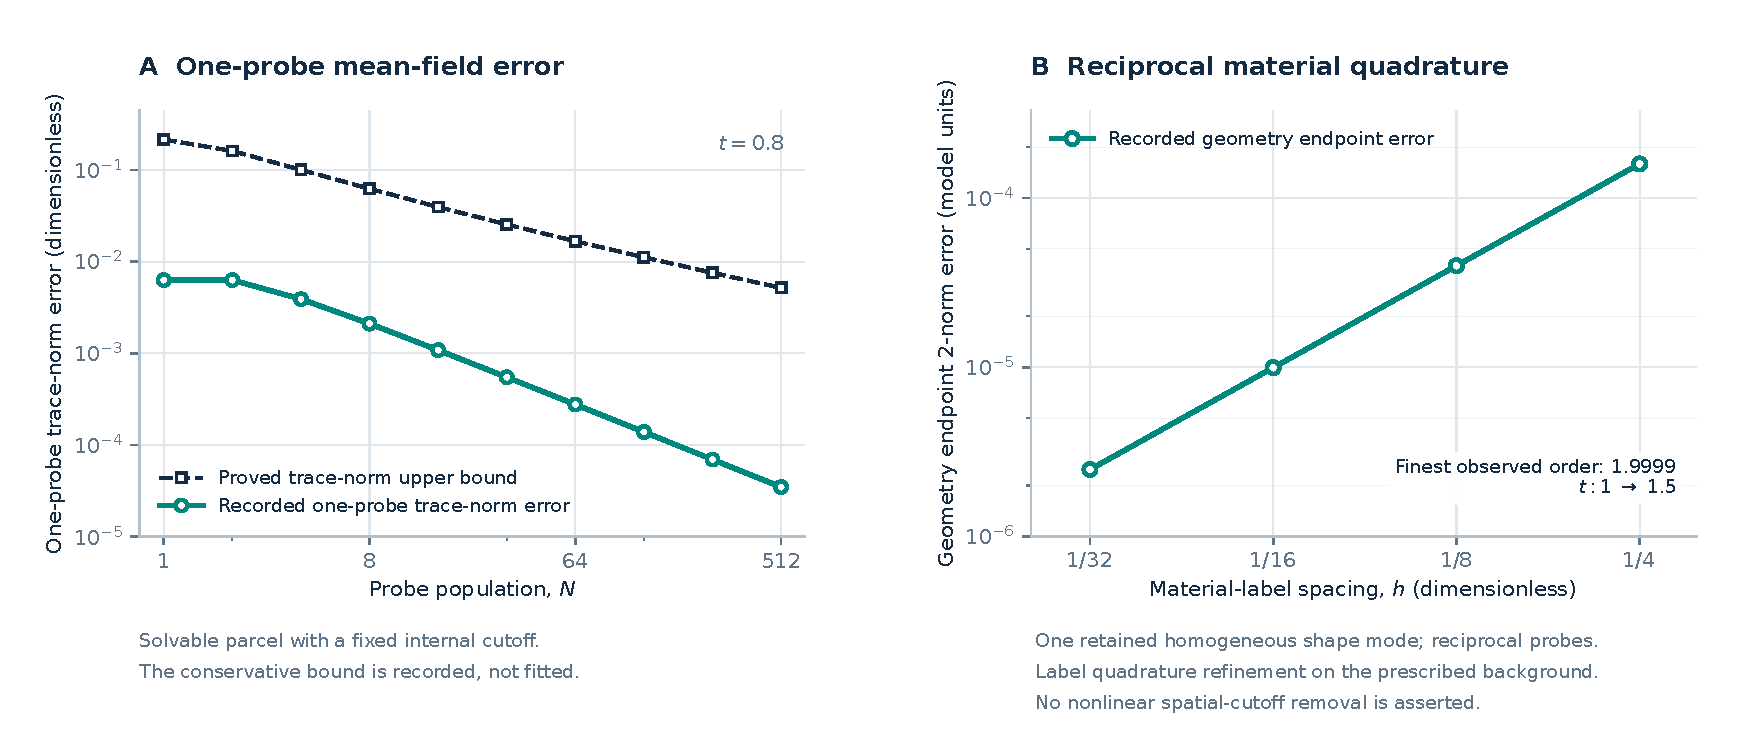
\includegraphics[width=\textwidth]{../figures/continuum.pdf}
\caption{Recorded controls. Left: exact-form one-probe errors and the proved bound for a solvable collective parcel. Right: nonlinear reciprocal material quadrature with one retained homogeneous shape mode on the prescribed background. The right panel does not remove the nonlinear geometric spatial cutoff.}
\end{figure}

The reciprocal material test reduces its geometry endpoint error from $1.59\times10^{-4}$ to $2.49\times10^{-6}$ with orders approaching two. The separate linearized spatial test for mode $(1,2)$ on $[1,2]$ gives orders 2.0105, 2.0028, and 2.0007, with every computed energy error below the analytic estimate. The internal-cutoff control retains the insufficient 24-level result and the improved 32-level result; printed floating-point zeros are not treated as exact identities.

\begin{center}\small
\begin{tabular}{@{}>{\raggedright\arraybackslash}p{0.50\textwidth}>{\raggedright\arraybackslash}p{0.43\textwidth}@{}}
\toprule
Evidence & Executed scope\\\midrule
Mean-field checker & 164 exact checks; parcel, clock, preparation, square-root, partial-trace, and source/lapse controls\\
Field/current checker & 92 exact checks; reciprocal quadrature, strong current/contact, tangent spatial, and Fock controls\\
Obstruction checker & 28 exact checks plus finite purity and collective-mass tests\\
Separate positive-chain review & 12 exact identities and 12 bounded controls\\
Lean project & 75 theorems in ten modules; zero warnings and errors\\\bottomrule
\end{tabular}
\end{center}

The 12 added Lean certificates prove explicit scalar estimate consequences and algebraic bookkeeping. They do not formalize the entire operator, fluid, or nonlinear convergence argument. The previous 63 theorem sources are unchanged. The project remains pinned to Lean 4.19.0 and the same mathlib revision; all axiom reports use the declared standard foundations, with true and false compiler controls.

The independent review corrected clock orientation, the global domain needed by the optional Hamilton--Jacobi argument, fluctuation-norm conversion, current ordering, and limit bookkeeping before public writing. This was separately tasked AI-assisted checking, not external human peer review. All tests are mathematical or synthetic.

\subsection{What is now connected}
The proved route is quantum collective dynamics to relativistic parcels, then reciprocal nonlinear matter continuum and strong current/contact convergence at fixed geometric basis. Ordered internal removal is available under its common-interval and weighted-regularity hypotheses. A separate tangent theorem establishes a smooth whole-field spatial limit.

The remaining obligation is specific: remove the nonlinear geometric cutoff with estimates strong enough for the full field equations, constraints, and local reconstruction. No unrestricted nonlinear Einstein-constraint limit, fixed-parameter interacting quantum-gravity continuum, or ordinary four-dimensional matter uplift is claimed. Existing mean-field, fluid, and semiclassical methods are credited~\cite{GMP,Chen,Dobrushin}; the contribution here is the explicit controlled construction and its verified boundaries in this selected-interaction framework.

\section*{Availability and reproduction}
The repository retains the preceding papers, the present proof notes, all source programs, execution receipts, raw control data, independent-review records, and phase-freeze hashes. Run the unified reproduction command from the repository root:
\begin{quote}\small\ttfamily
python scripts/reproduce.py --output-dir work/reproduction
\end{quote}
The formal verifier is run separately after preparing the pinned dependencies. Research by Logan Voss, with AI-assisted derivation, verification, formalization, and editing.

\begin{thebibliography}{8}
\bibitem{Voss2} L. Voss, \emph{On Quantum Mechanics and General Relativity: Dynamical Extensions}, research edition 2.0 (2026). \href{https://github.com/LoganVoss/on-quantum-mechanics-and-general-relativity/releases/tag/v2.0.1}{Preserved release}.
\bibitem{Brown} J. D. Brown, \emph{Action functionals for relativistic perfect fluids}, Class. Quant. Grav. 10, 1579--1606 (1993). \href{https://arxiv.org/abs/gr-qc/9304026v1}{arXiv:gr-qc/9304026v1}.
\bibitem{GMP} F. Golse, C. Mouhot, T. Paul, \emph{On the Mean Field and Classical Limits of Quantum Mechanics} (2015). \href{https://arxiv.org/abs/1502.06143}{arXiv:1502.06143}.
\bibitem{Chen} X. Chen, S. Shen, Z. Zhang, \emph{On the mean-field and semiclassical limit from quantum N-body dynamics}. \href{https://arxiv.org/abs/2304.03447}{arXiv:2304.03447}.
\bibitem{Dobrushin} R. L. Dobrushin, \emph{Vlasov equations}, Funct. Anal. Appl. 13 (1979). \href{https://doi.org/10.1007/BF01077243}{doi:10.1007/BF01077243}.
\bibitem{LionsPaul} P.-L. Lions, T. Paul, \emph{Sur les mesures de Wigner}, Rev. Mat. Iberoam. 9 (1993). \href{https://ems.press/journals/rmi/articles/5283}{Primary journal article}.
\bibitem{Hardy} E. Berchio, D. Ganguly, G. Grillo, \emph{Sharp Poincaré-Hardy and Poincaré-Rellich inequalities on the hyperbolic space}. \href{https://arxiv.org/abs/1507.02550v4}{arXiv:1507.02550v4}.
\bibitem{Hackl} L. Hackl, E. Bianchi, \emph{Bosonic and fermionic Gaussian states from Kähler structures}, SciPost Phys. Core 4, 025 (2021). \href{https://arxiv.org/abs/2010.15518v4}{arXiv:2010.15518v4}.
\end{thebibliography}
\end{document}
